\documentclass[12pt, letterpaper]{article}

\usepackage{url}

%Line Spacing
\usepackage{setspace}
\doublespacing

%Graphics
\usepackage{graphicx}

%Margins
\usepackage[margin=1in]{geometry}

%Citations
\usepackage[backend=biber,style=ieee,urldate=long]{biblatex}
\addbibresource{./refs.bib}

%Figures
\usepackage{float}

\title{Passwordless Authentication}
\author{Zachary Thompson}

\begin{document}
\maketitle

\section{Executive Summary}
This paper will analyze passwordless authentication.
It will first examine various flaws with traditional, password-based authentication.
Then, the paper will discuss how passwordless authentication addresses those flaws and provide an example of the system in action.
After that, there will be a discussion of how account recovery could work with a passwordless authentication system, and it will look at some of the flaws with such a system.
Finally there will be analysis and recommendations regarding what further research can be done and whether users should consider switching to passwordless authentication.


\newpage
\section{Introduction}
Passwords have been the main way we authenticate users for many years now, but, with issues like password reuse, data breaches, and phishing, is there some more secure way we could perform authentication?
Widespread access to devices like smartphones is increasing the number of ways to authenticate users.

Passwordless authentication describes a collection of authentication methods which do not rely on the user remembering and entering a password in order to be authenticated.
Proponents of passwordless authentication argue it is both more convenient and secure than traditional, password-based authentication.

With large corporations like Microsoft and Google embracing a move to passwordless authentication, we need to evaluate whether this really is the right direction to move in \parencite{msftpaswdless}, \parencite{googpaswdless}.

\newpage
\section{Discussion}

\subsection{The Problem With Passwords}
Password-based authentication has a number of glaring flaws.
For one, passwords are prone to reuse.
It is difficult to remember dozens of unique passwords, so people end up using the one they already memorized over and over again.
According to a poll conducted by Google and Harris in 2019, 52\% of people reuse a password for multiple accounts and 13\% reused a password for all of their accounts \parencite{googleharris2019poll}.
Password reuse leaves other accounts which use the same or a similar password vulnerable to attack.
If an attacker were to compromise one password, then there is a good chance they could use it to breach other accounts.

Another problem is that good passwords are difficult to memorize.
Good passwords are long and use different types of symbols.
Ideally, a password would be a long, randomly generated string of characters.
A password like that is hard enough to memorize for one website, let alone all of the ones we use.
It is unreasonable to expect users to remember many unique and strong passwords.

Password managers help in this regard.
They are able to generate and store strong passwords for you.
This means that, assuming the password manager is used correctly, all of your passwords will be difficult to crack and will be unique. 
However, all of your passwords are now only as strong as your master password (and the security of your password manager).
One strong password is likely better than a hundred weak ones, but it probably isn't a good idea to put all your eggs in one basket.

Passwords are particularly vulnerable to any sort of attack which involves the attacker stealing the password instead of guessing it.
A common example of this type of attack is phishing: the attacker tricks the user into entering their password by sending them a deceptive message.
Phishing was the most common type of cyber crime in 2020 and a password manager will not defend against this type of attack \parencite{fbi2020icr}.
Another way an attacker could steal a password is through a data breach.
The website haveibeenpwned.com, which keeps track of leaked credentials, has over 613 million revealed passwords in its records \parencite{hibpweb}.
And with password reuse being common, the attacker could use the leaked passwords to attack many more accounts than just those associated with the leak.

Clearly passwords have a number of flaws which need to be addressed.
81\% of hacking-related security breaches in 2017 involved stolen or weak passwords, so there is plenty of reason to look for an alternative authentication method \parencite{verizon2017dbir}.

\subsection{A Solution: Get Rid of the Password}
Perhaps the way to eliminate the problems of passwords is to not use passwords at all and instead use some other form of authentication.
That is exactly what Microsoft allows you to do with your Microsoft account using their Authenticator app. 

\begin{figure}[h]
\centering
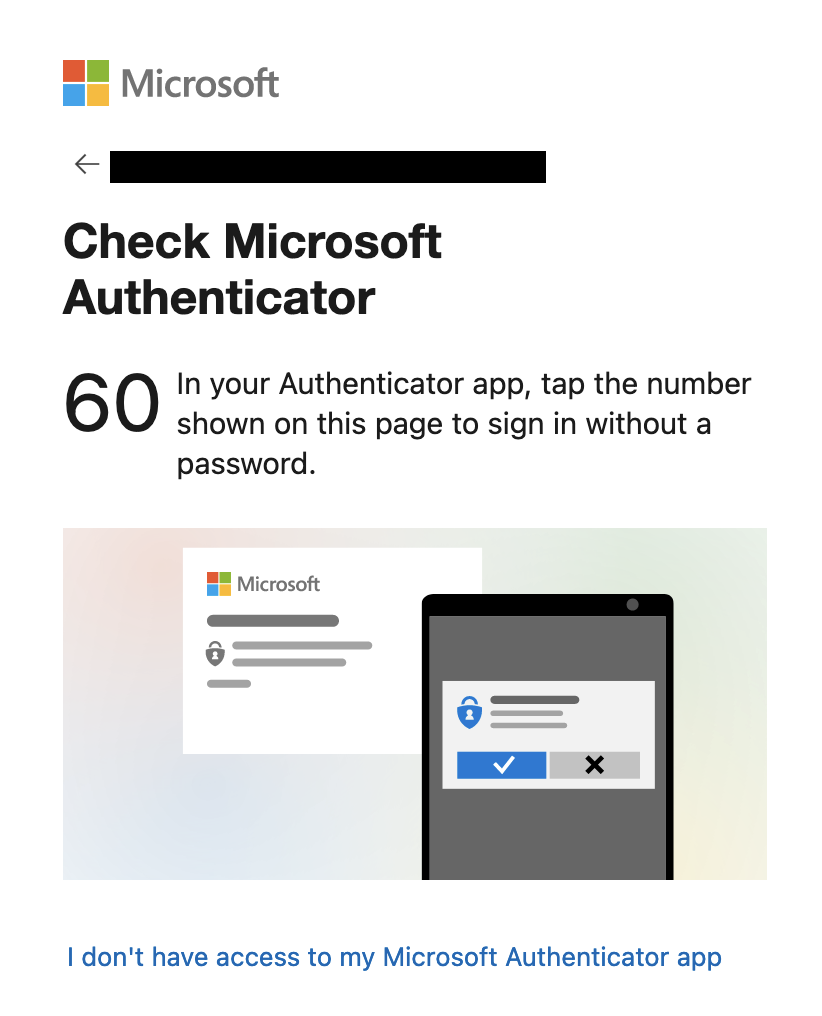
\includegraphics[width=0.4\textwidth]{mslogin.png}
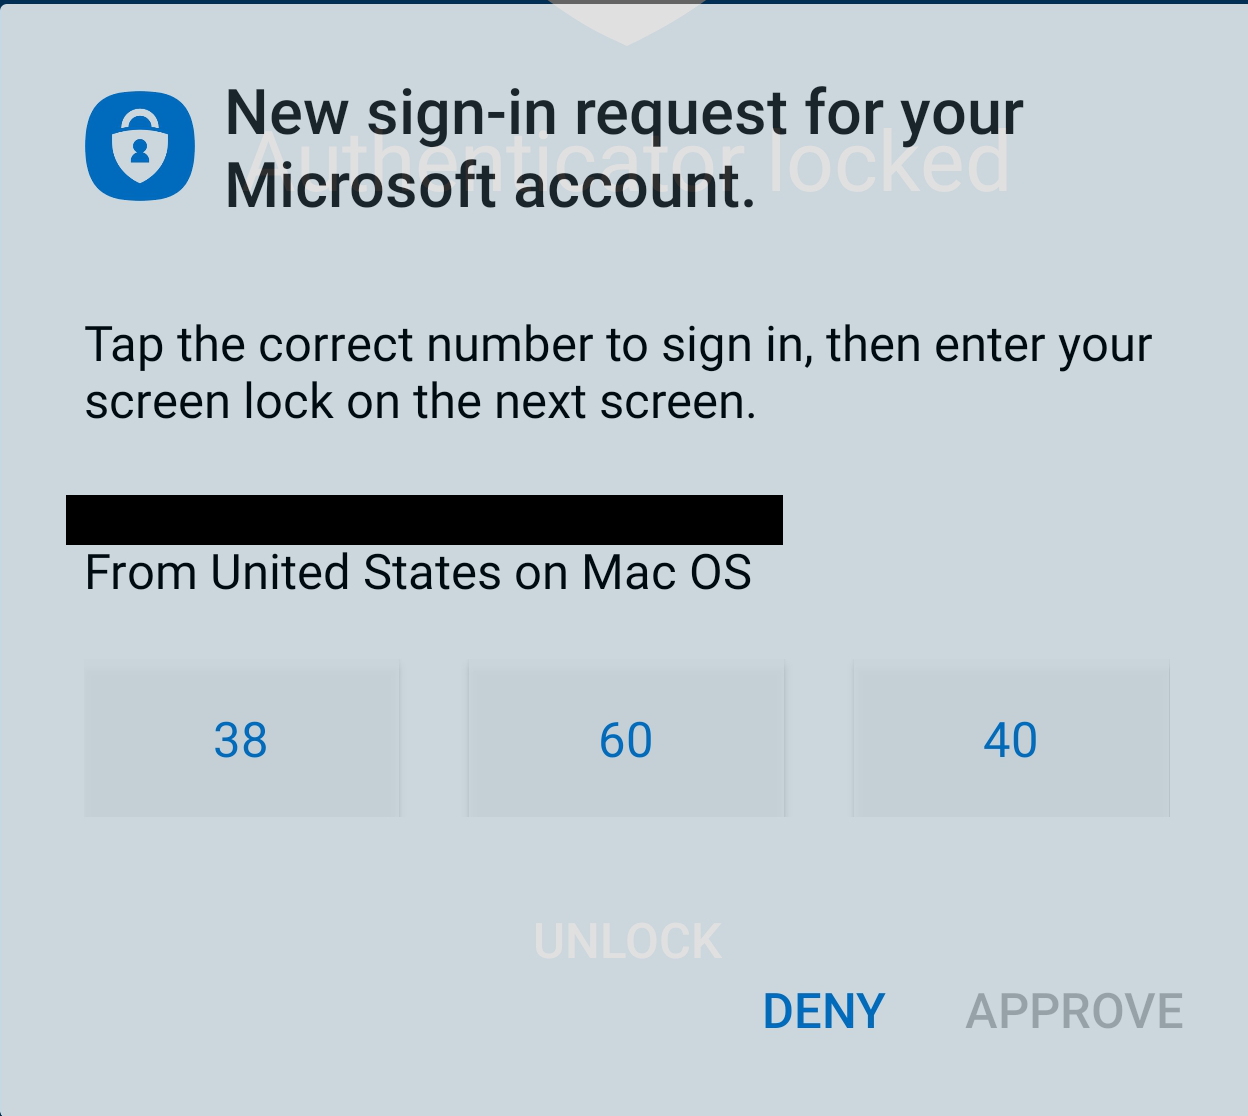
\includegraphics[width=0.4\textwidth]{authenticator.png}
\caption{Microsoft's Passwordless Authentication\label{msauth}}
\end{figure}

Figure \ref{msauth} shows Microsoft's passwordless authentication system.
Every time you login to your Microsoft account, you will get a prompt on your phone which will ask you to select the same number that is displayed on the device you wish to log into.
As long as you have your phone near you, it is a quick and easy process, especially on devices without a physical keyboard such as Microsoft's Xbox.

A passwordless authentication scheme does not have to work exactly like Microsoft's where the user needs to use a smartphone app; it could also use biometrics or some type of smart token.
In fact, any of these methods can be combined to have much stronger, multi-factor authentication.

This type of system is not vulnerable to any of the flaws that were discussed earlier with passwords.
The user does not have to remember anything, they simply need to have access to the token that they set up.
Phishing attacks are virtually impossible since the user can't be tricked into entering a string.
Also, since their are no credentials to store, the user does not have to worry about data breaches.

\subsection{Account Recovery\label{recov}}
If the user is no longer able to access their authentication method (e.g. they lose their phone), then there needs to be some form of account recovery so that the user can fix the issue.

There are many potential ways to facilitate account revovery with a passwordless authentication system.
According to \parencite{kunke2021evaluation}, their analysis found that the strongest, currently in use mechanism was setting up a backup token with the service you wish to log into.
When the primary token is lost, then the backup token could be used to get into the account and reset the primary token.

There is also another method they mention known as pre-emptive syncing.
To put it simply, a backup authenticator syncs with a primary authenticator before passwordless authentication is set up.
When the primary authenticator is lost, then the user syncs the backup authenticator to the new primary authenticator and the user should be able to log in normally.
This method is currently only theoretical, but the researchers claim it is the most promising method in terms of security any usability.

\subsection{Potential Problems}
Passwordless authentication does have a few problems that can arise.
First is that the account recovery described in section \ref{recov} is less convenient than account recovery in password-based authentication.
Setting up a backup token for every website can be tedious.
However, clicking the ``reset password'' link and following the steps listed by the website is usually a simple process as long as the user has access to their email.

There is also the financial cost of switching to a passwordless authentication system.
Companies will have to invest money into developing their websites to support passwordless authentication and the associated recovery methods.
There may also be costs with purchasing hardware tokens, although this can largely be avoiding by using smartphones along with their biometric scanners.
\newpage
\section{Analysis and Recommendations}
Passwordless authentication is something ordinary people and businesses should seriously consider utilizing.
With smartphones, it should be fairly easy to enable it with any website that offers it.
Check and see if services you use support this method of authentication and determine if it is something you feel is more convenient and secure.

For accounts where passwordless authentication is not an option, consider using a password manager to generate and store strong passwords and minimize password reuse.
Remember to make your master password very strong!

In regards to account recovery, more research needs to be done.
The analysis in \parencite{kunke2021evaluation} mentions multiple theoretical methods of account recovery which have not been implemented.
These methods, especially pre-emptive syncing need to be studied and tested to see whether they may be a more secure and/or convenient form of account recovery.

\newpage
\section{Conclusion}
All in all passwordless authentication is a promising solution to the shortcomings of password-based authentication.
Passwords have problems related to reuse, the need to memorize, and theft.
Passwordless authentication does not suffer from any of these problems while generally being a convenient way to login to a service.
It does have some drawbacks, namely the inconvenient methods for account recovery and the cost to implement.

Passwordless authentication is an option every one should know about and consider using.
It has the potential to save many users from the most common cyber attacks while also making signing into websites easier.

\newpage
\printbibliography
\end{document}
